% 第三部分 A 结果：GRPO 训练（由 main_zh.tex 引入）。

\section{针对可见测试的训练}\label{sec:res-grpo}

每种奖励训练策略 100 步（每步 16 道题、每题 8 个回合，学习率 $10^{-5}$，与第二部分相同），各用 \NUM{cgseeds_vis} 个种子。表~\ref{tab:code-grpo} 给出最终策略在三个评估集上的结果，表~\ref{tab:code-paired} 给出奖励之间的配对差，图~\ref{fig:code-curves} 给出训练曲线。95\% 区间按题目重采样，不包含种子之间的差异，因此在种子结果不一致的地方，我们也给出每个种子的数值。

\paragraph{用可见测试训练让代码更正确。} 第 0 步时，基座策略在 \NUM{cgszmean_kod_allpass}\% 的 KodCode val 题目、\NUM{cgszmean_mbpp_allpass}\% 的 MBPP+ 题目和 \NUM{cgszmean_he_allpass}\% 的 HumanEval+ 题目上通过全部测试。用 \texttt{vis} 奖励训练 100 步后，这三个比例为 \NUM{cgall_vis_kod}\%、\NUM{cgall_vis_mbpp}\% 和 \NUM{cgall_vis_he}\%，而且需要的修复更少：它在首次尝试就解出 \NUM{cgfirst_vis_kod}\% 的 KodCode val 题目，第 0 步时为 \NUM{cgszmean_kod_firstattemptallpass}\%。MBPP+ 和 HumanEval+ 从未用于训练。

\paragraph{可见测试与留出测试之间的差距在两个集合上缩小了，在 MBPP+ 上没有。} 在基座策略于 KodCode val 上通过可见测试的尝试中，有 \NUM{cgszmean_kod_hackamongvispass}\% 在留出测试上失败；训练后为 \NUM{cghackv_vis_kod}\%。在 HumanEval+ 上，这一比例从 \NUM{cgszmean_he_hackamongvispass}\% 降到 \NUM{cghackv_vis_he}\%。在 MBPP+ 上它几乎不变，从 \NUM{cgszmean_mbpp_hackamongvispass}\% 到 \NUM{cghackv_vis_mbpp}\%：策略通过 MBPP+ 可见测试的题目多了很多（第 0 步为 \NUM{cgszmean_mbpp_vispass}\%，训练后为 \NUM{cgvis_vis_mbpp}\%），而可见测试通过、留出测试失败的题目占全部题目的比例从 \NUM{cgszmean_mbpp_hack}\% 增加到 \NUM{cghack_vis_mbpp}\%。训练没有让策略对可见测试的过拟合比基座策略更严重；但在 MBPP+ 上，也没有让它减轻。

\begin{table}[t]
\centering\small
\begin{tabular}{@{}lcccccccccc@{}}
\toprule
 & & \multicolumn{3}{c}{KodCode val} & \multicolumn{3}{c}{MBPP+} & \multicolumn{3}{c}{HumanEval+} \\ \cmidrule(lr){3-5}\cmidrule(lr){6-8}\cmidrule(lr){9-11}
condition & seeds & vis & all & hack & vis & all & hack & vis & all & hack \\ \midrule
\texttt{vis} & 2 & 97.1 & 86.6 & 10.6 & 84.7 & 69.3 & 15.4 & 88.5 & 76.4 & 12.1 \\
\texttt{vis\_kev} & 2 & 96.6 & 86.6 & 10.1 & 85.2 & 72.3 & 12.9 & 87.9 & 76.7 & 11.2 \\
\texttt{hidden} & 2 & 96.3 & 87.2 & 9.1 & 82.0 & 68.8 & 13.3 & 88.2 & 77.0 & 11.2 \\
\bottomrule
\end{tabular}

\caption{最终策略（贪心解码，最多三次尝试）：通过可见测试（\emph{vis}）、通过全部测试（\emph{all}），以及通过可见测试但有留出测试失败（\emph{hack}）的题目比例（\%）；种子均值。}
\label{tab:code-grpo}
\end{table}

\paragraph{预言机奖励：错误的通过略少，解出的题目没有增加。} \texttt{hidden} 只奖励通过全部测试的代码，因此从不奖励错误的程序。它的最终策略解出的题目与 \texttt{vis} 一样多：all pass 的差值在 KodCode val 上为 \NUM{cgdall_hidden_kod} \ci{\NUM{cgdalllo_hidden_kod}}{\NUM{cgdallhi_hidden_kod}} 个百分点，在 MBPP+ 上为 \NUM{cgdall_hidden_mbpp} \ci{\NUM{cgdalllo_hidden_mbpp}}{\NUM{cgdallhi_hidden_mbpp}}，在 HumanEval+ 上为 \NUM{cgdall_hidden_he} \ci{\NUM{cgdalllo_hidden_he}}{\NUM{cgdallhi_hidden_he}}（表~\ref{tab:code-paired}）。它通过可见测试的频率更低（MBPP+ 上为 \NUM{cgvis_hidden_mbpp}\%，\texttt{vis} 为 \NUM{cgvis_vis_mbpp}\%），而差异的大部分来自错误的程序：hack 率的差值分别为 \NUM{cgdhack_hidden_kod} \ci{\NUM{cgdhacklo_hidden_kod}}{\NUM{cgdhackhi_hidden_kod}}、\NUM{cgdhack_hidden_mbpp} \ci{\NUM{cgdhacklo_hidden_mbpp}}{\NUM{cgdhackhi_hidden_mbpp}} 和 \NUM{cgdhack_hidden_he} \ci{\NUM{cgdhacklo_hidden_he}}{\NUM{cgdhackhi_hidden_he}} 个百分点，只有在 MBPP+ 上区间不含零。
一个从不奖励错误程序的奖励，让其中一部分不再通过可见测试；但在 100 步之内，它没有把它们变成正确的程序。

\begin{table}[t]
\centering\small
\begin{tabular}{@{}lcccccc@{}}
\toprule
 & \multicolumn{3}{c}{all pass} & \multicolumn{3}{c}{hack} \\ \cmidrule(lr){2-4}\cmidrule(l){5-7}
minus \texttt{vis} & KodCode val & MBPP+ & HumanEval+ & KodCode val & MBPP+ & HumanEval+ \\ \midrule
\texttt{vis\_kev} & $+$0.0 & $+$3.1 & $+$0.3 & $-$0.5 & $-$2.5 & $-$0.9 \\
 & {\footnotesize \ci{$-$2.5}{2.5}} & {\footnotesize \ci{1.1}{5.2}} & {\footnotesize \ci{$-$3.7}{4.3}} & {\footnotesize \ci{$-$2.9}{1.7}} & {\footnotesize \ci{$-$4.5}{$-$0.7}} & {\footnotesize \ci{$-$3.7}{1.9}} \\[2pt]
\texttt{hidden} & $+$0.7 & $-$0.5 & $+$0.6 & $-$1.5 & $-$2.1 & $-$0.9 \\
 & {\footnotesize \ci{$-$1.8}{3.2}} & {\footnotesize \ci{$-$2.5}{1.3}} & {\footnotesize \ci{$-$3.4}{5.0}} & {\footnotesize \ci{$-$3.9}{0.8}} & {\footnotesize \ci{$-$4.0}{$-$0.3}} & {\footnotesize \ci{$-$4.7}{2.8}} \\[2pt]
\bottomrule
\end{tabular}

\caption{相对 \texttt{vis} 的配对差（百分点）：在每道题上取各条件的种子均值，求差后对题目取平均，并给出按题目重采样的 95\% 区间。}
\label{tab:code-paired}
\end{table}

\paragraph{评判因子：对 MBPP+ 的作用只出现在一个种子中。} \texttt{vis\_kev} 把可见测试奖励乘以 \kev{} 的 \emph{genuine} 分数。在 KodCode val 和 HumanEval+ 上，它的最终策略解出的题目与 \texttt{vis} 一样多（\NUM{cgdall_viskev_kod} \ci{\NUM{cgdalllo_viskev_kod}}{\NUM{cgdallhi_viskev_kod}} 和 \NUM{cgdall_viskev_he} \ci{\NUM{cgdalllo_viskev_he}}{\NUM{cgdallhi_viskev_he}}）。在 MBPP+ 上种子均值更好：all pass 的差值为 \NUM{cgdall_viskev_mbpp} \ci{\NUM{cgdalllo_viskev_mbpp}}{\NUM{cgdallhi_viskev_mbpp}} 个百分点，hack 率的差值为 \NUM{cgdhack_viskev_mbpp} \ci{\NUM{cgdhacklo_viskev_mbpp}}{\NUM{cgdhackhi_viskev_mbpp}}，按题目的区间不含零。但两个种子并不一致：\texttt{vis\_kev} 在种子 1 下通过 \NUM{cgall_viskev_mbpp_s1}\% 的 MBPP+ 题目的全部测试，在种子 2 下为 \NUM{cgall_viskev_mbpp_s2}\%，而 \texttt{vis} 分别为 \NUM{cgall_vis_mbpp_s1}\% 和 \NUM{cgall_vis_mbpp_s2}\%。两个种子中只有一个出现的效果，不是我们能够宣称的效果。

\paragraph{没有抄写测试。} hack 率统计每一个通过可见测试的错误程序，不论它只是不完整，还是对测试做了特判。为了区分两者，我们寻找最粗暴的特判形式：程序中出现了可见测试里的某个值（参数或期望结果），而参考解答中没有这个值（\file{dcjev/analysis/code_hacks.py}；只搜索被测函数及其用到的模块级代码，因此模型自己写的示例调用不算）。这项检查标出了离线研究中 \NUM{ch_hardcoded_n} 个硬编码查表程序中的 \NUM{ch_hardcoded_copy} 个，即每一个含有非平凡值的查表程序，而 \NUM{ch_reference_n} 个参考解答一个也没有标出。在离线研究中基座策略的尝试里，它标出了 \NUM{ch_policyhack_n} 个通过可见测试但有留出测试失败的尝试中的 \NUM{ch_policyhack_copy} 个，以及其余尝试的 \NUM{ch_policyother_frac}。训练期间，在 \texttt{vis} 的任何一个十步窗口中，它最多标出 \NUM{ch_max_vis} 的回合（\texttt{vis\_kev} 为 \NUM{ch_max_viskev}，\texttt{hidden} 为 \NUM{ch_max_hidden}），且没有上升趋势（表~\ref{tab:code-copies}）。在最终评估中，它标出了 \texttt{vis} 的 \NUM{ch_finhackn_vis} 个 hack 回合中的 \NUM{ch_finhack_vis} 个、\texttt{vis\_kev} 的 \NUM{ch_finhackn_viskev} 个中的 \NUM{ch_finhack_viskev} 个，以及 \texttt{hidden} 的 \NUM{ch_finhackn_hidden} 个中的 \NUM{ch_finhack_hidden} 个。通过可见测试的错误程序几乎从不含有测试中的值，训练前后都是如此；可见测试奖励没有教会策略抄写测试。不抄写任何值的特判，这项检查发现不了。

\begin{table}[t]
\centering\small
\begin{tabular}{@{}lcccccc@{}}
\toprule
 & & \multicolumn{3}{c}{training episodes that copy} & \multicolumn{2}{c}{final evaluation, copy} \\ \cmidrule(lr){3-5}\cmidrule(l){6-7}
condition & seeds & steps 0--9 & steps 50--59 & steps 90--99 & hack & all pass \\ \midrule
\texttt{vis} & 2 & 0.2\% & 0.2\% & 0.0\% & 1 / 218 & 2 / 1283 \\
\texttt{vis\_kev} & 2 & 0.2\% & 0.1\% & 0.0\% & 0 / 193 & 1 / 1307 \\
\texttt{hidden} & 2 & 0.2\% & 0.0\% & 0.0\% & 0 / 190 & 4 / 1285 \\
\bottomrule
\end{tabular}

\caption{含有参考解答中没有的可见测试值的程序：三个十步窗口中训练回合的比例（种子均值），以及最终评估的 hack 回合和 all pass 回合中的数量（所有种子和评估集合计）。}
\label{tab:code-copies}
\end{table}

\begin{figure}[t]
\centering
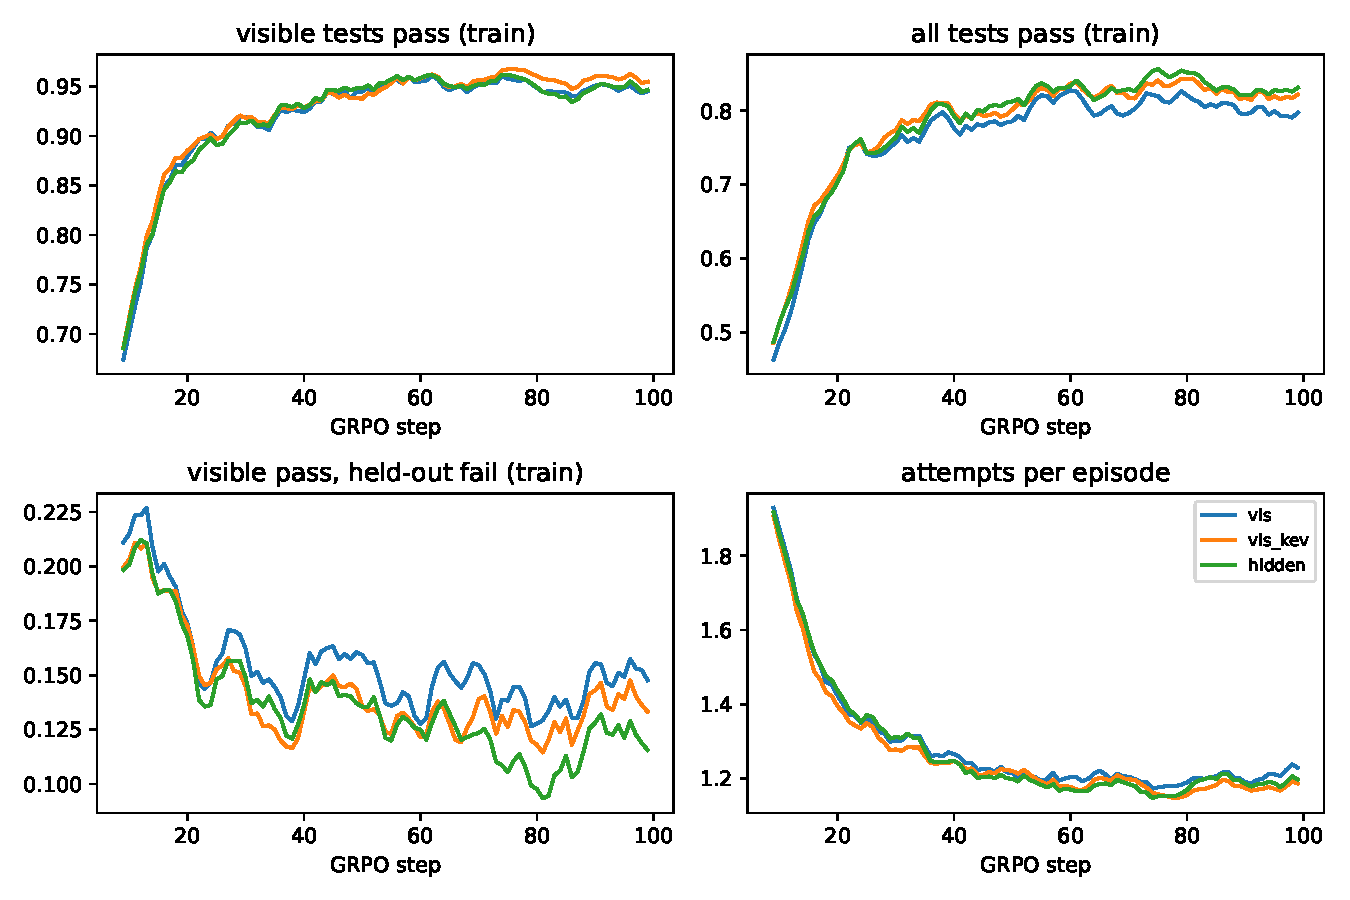
\includegraphics[width=\linewidth]{../../experiments/part3a_code/results/training_curves.pdf}
\caption{训练曲线（种子均值，10 步滑动平均）：训练回合中通过可见测试、通过全部测试、通过可见测试但有留出测试失败的比例，以及每个回合的尝试次数。}
\label{fig:code-curves}
\end{figure}

\paragraph{评估噪声。} 每次运行都在第 0 步评估同一个基座模型。在 \NUM{cgszruns_kod_allpass} 次运行中，KodCode val 上的 all pass 介于 \NUM{cgszmin_kod_allpass}\% 和 \NUM{cgszmax_kod_allpass}\% 之间（标准差 \NUM{cgszsd_kod_allpass} 个百分点），MBPP+ 上介于 \NUM{cgszmin_mbpp_allpass}\% 和 \NUM{cgszmax_mbpp_allpass}\% 之间，HumanEval+ 上介于 \NUM{cgszmin_he_allpass}\% 和 \NUM{cgszmax_he_allpass}\% 之间。vLLM 上的贪心解码在不同的服务器状态下不能逐位复现。同一奖励不同种子之间的差异更大：all pass 的标准差最高达 \NUM{cgallsd_viskev_mbpp} 个百分点（\texttt{vis\_kev}，MBPP+）。
